\documentclass[final]{beamer}
%define logos
\def\RightLogoWidth{0.7}
\def\LeftLogo{/Users/willbarnes/Documents/Rice/Posters/spd_poster_contest.jpg}
\def\LeftLogoWidth{2.3}
\def\RightLogo{/Users/willbarnes/Documents/Rice/Posters/RiceLogo_TMCMYK300DPI.jpg}
\mode<presentation>
{
\usetheme{I6dv}
}
\setbeamertemplate{caption}[numbered]
%Include packages
\usepackage{type1cm}
\usepackage{calc} 
\usepackage{times}
\usepackage{amsmath,amsthm, amssymb, latexsym}
\usepackage{epstopdf}
\usepackage[numbers]{natbib}
\usepackage{subfigure}
\usepackage[english]{babel}
\usepackage[latin1]{inputenc}
\usepackage[orientation=portrait,size=custom,width=91.44,height=106.68,scale=1.4,debug]{beamerposter}
%Define new commands here
\newcommand{\ang}{\AA~}
%Set author and title
\title[NMF in Active Regions]{Nonnegative Matrix Factorization as a Tool\\for Improved Event Detection in Active Region Cores}
\author[Barnes \& Bradshaw]{Will T. Barnes \& Stephen J. Bradshaw}
\institute[Rice University]{Department of Physics and Astronomy, Rice University}
\date{26-30 April, 2015}
%Start poster
\begin{document}
\begin{frame}{} 
    \begin{columns}[t]
		\hfill
		\hfill
		%start first column
      \begin{column}{.32\linewidth}
		  %Begin intro section
        \begin{block}{Introduction}
          \begin{itemize}
			  \item Determining the \alert{frequency of energy release} in active regions (ARs) is a critical step toward learning how the solar corona is powered.
			  \item Vast amounts of data $\rightarrow$ need for improved techniques for identifying impulsive heating signatures
			  \item \textbf{Goal:} Predict heating frequency in AR cores using \alert{nonnegative matrix factorization (NMF)} to analyze intensity fluctuations in forward-modeled pixel-averaged light curves
		  \end{itemize}
        \end{block}
		%Begin nanoflare block
		\begin{block}{Nanoflare Signatures}
			\begin{itemize}
				\item Nanoflares \citep{parker_nanoflares_1988} are a strong candidate for the mechanism behind coronal heating
				\item Observational signatures difficult to detect$\rightarrow$ short timescale, non-equilibrium ionization, etc.
				\item \alert{Single peak may be convolution of many nanoflare signatures;} counting methods not able to resolve these sources.
			\end{itemize}
			\begin{figure}
				\subfigure[]{%
				\includegraphics[width=0.49\columnwidth]{figures/obs_aia_94.eps}
				\label{fig:ar_viz_obs}}
				\subfigure[]{%
				\includegraphics[width=0.49\columnwidth]{figures/fm_aia_335.eps}
				\label{fig:ar_viz_fm}}
				\subfigure[]{%
				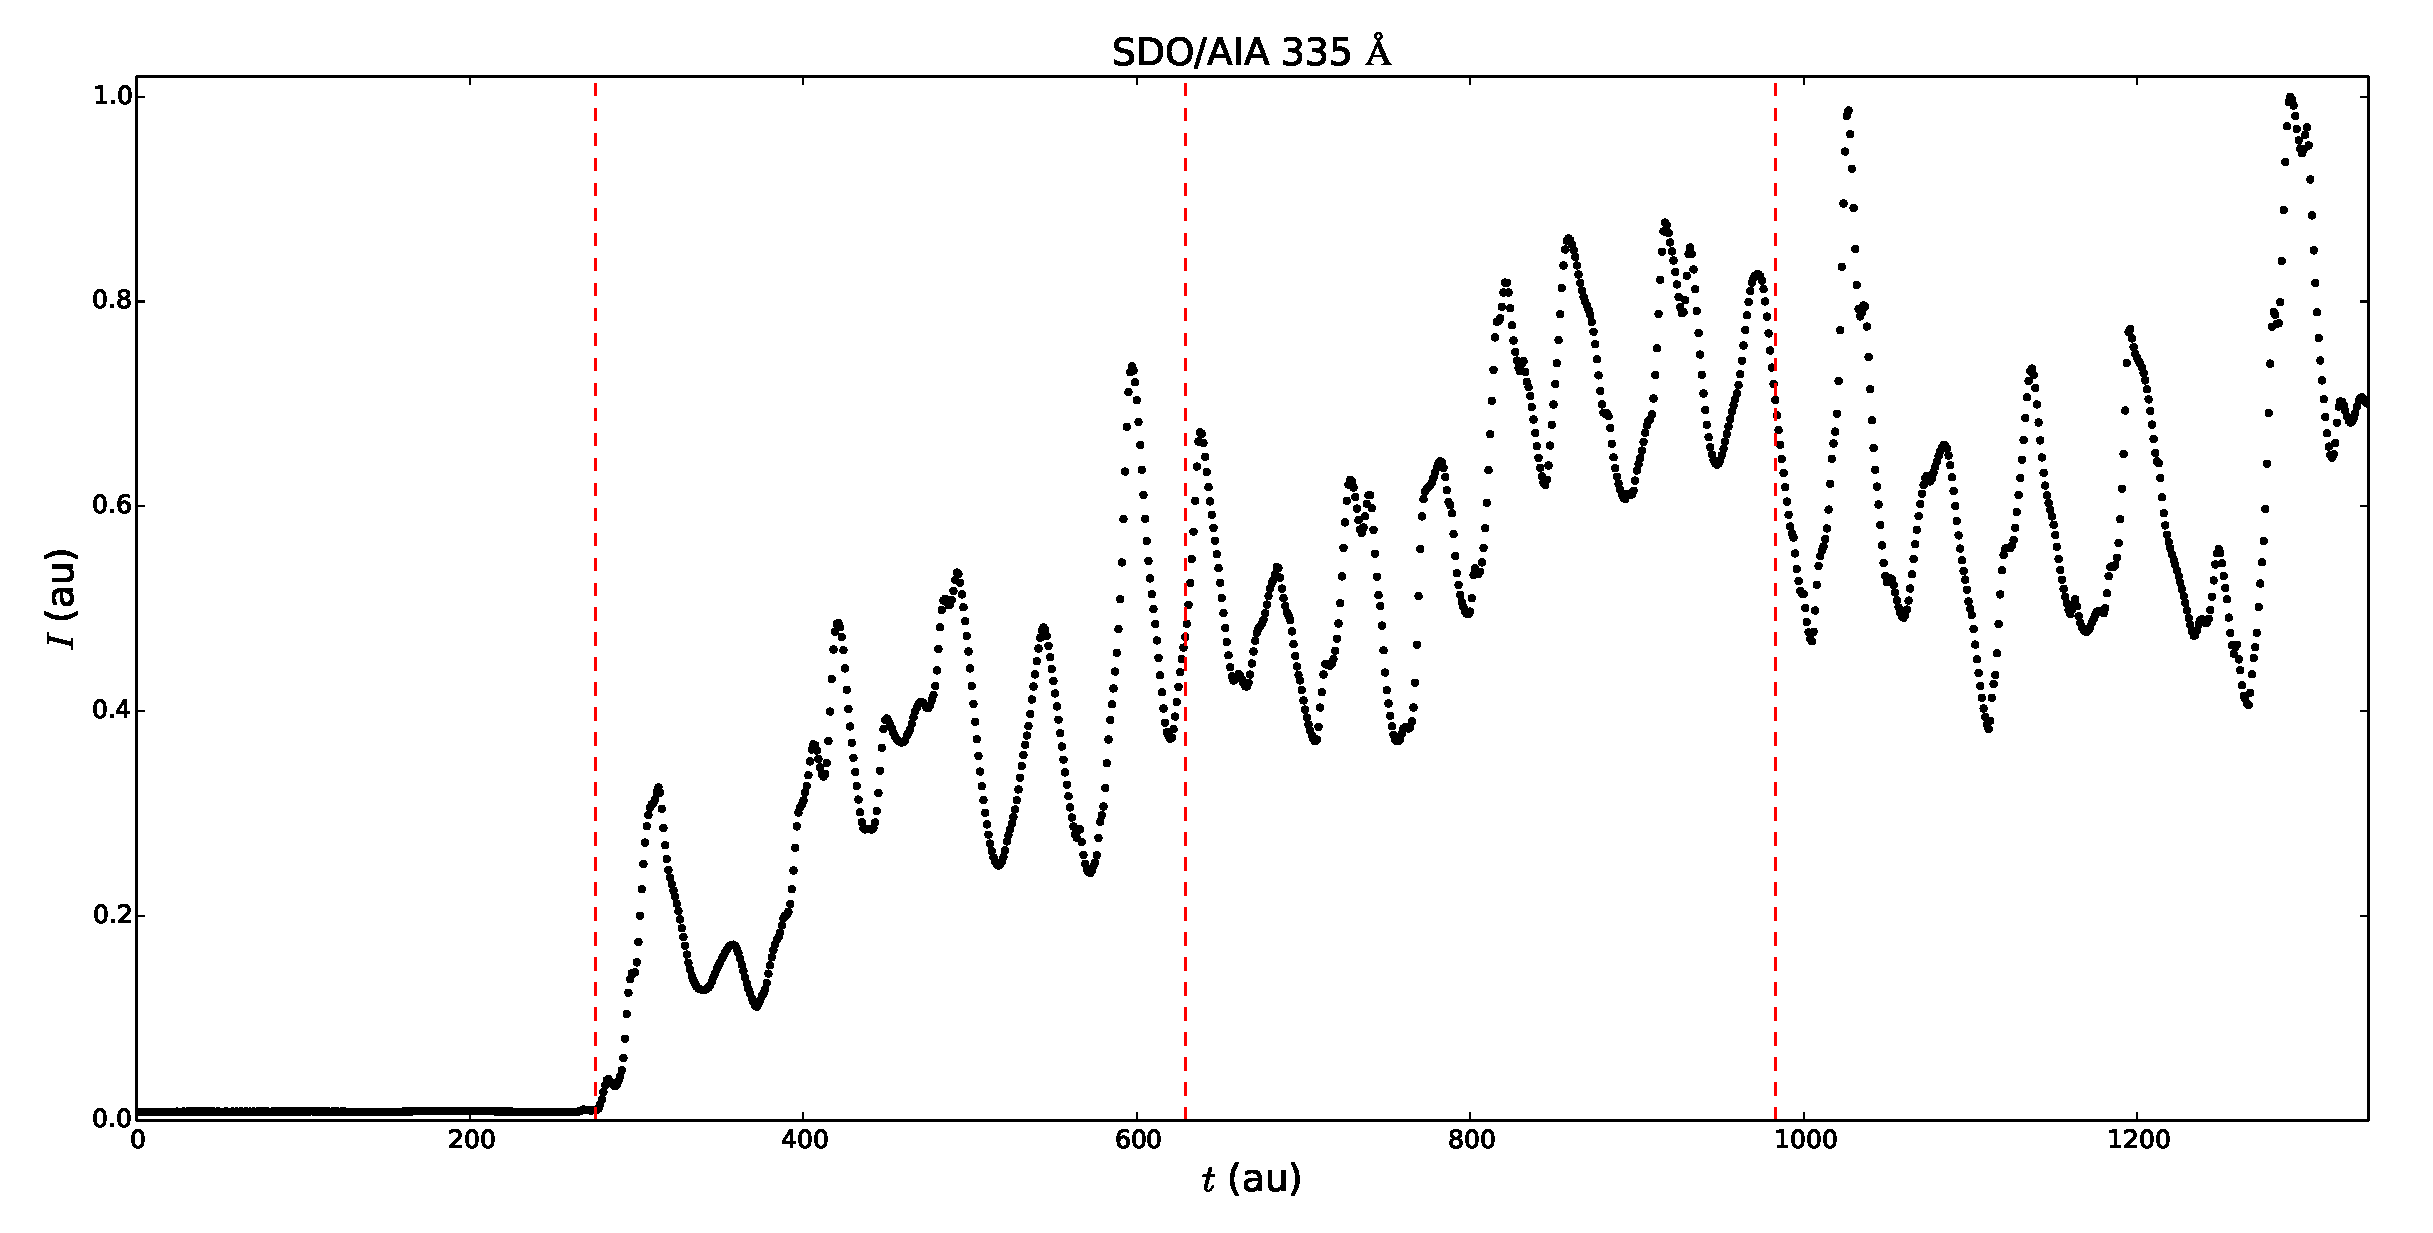
\includegraphics[width=0.98\columnwidth]{figures/ts_fm_335_aia.eps}
				\label{fig:ar_viz_ts}}
				\caption{\footnotesize\ref{fig:ar_viz_obs} SDO/AIA 94 \ang image of AR NOAA 11459 from 22 May 2012, 00:02 UT. \ref{fig:ar_viz_fm} Forward-modeled AR as seen by SDO/AIA 335 \ang subject to a total of $\sim$4000 nanoflares. The white box shows the region over which the pixel-averaged time series was calculated. \ref{fig:ar_viz_ts} Normalized time series calculated from pixel intensity inside white box of \ref{fig:ar_viz_fm}. Red lines show the different sections over which the factorization was performed.}
				\label{fig:ar_viz}
			\end{figure}
		\end{block}
		%Begin forward modeling block
		\begin{block}{Forward-modeling of AR Emission}
			\begin{itemize}
				\item Forward-modeled emission provides \alert{ideal proof of concept} for event detection algorithms
				\item Synthesized emission produced using $n$ and $T$ profiles from 1D hydrodynamic model HYDRAD \citep{bradshaw_influence_2013} coupled with forward modeling code \citep{bradshaw_what_2011,reep_diagnosing_2013}.
				\item Resulting intentisity can be mapped to 3D field line extrapolations \citep[e.g.][]{warren_static_2007} and the observed pixel intensity inferred from the integrated line-of-sight volumetric emission
			\end{itemize}
		\end{block}
		%%
      \end{column}
	  %start second column
      \begin{column}{.32\linewidth}
		  %%
  		%NMF advantages block
  		\begin{block}{Advantages of NMF}
  			\begin{itemize}
  				\item Active algorithm development and testing by resarchers in a variety of fields \citep[e.g. computational neuroscience, see][]{cichocki_nonnegative_2009,soelter_automatic_2014}
  				\item \alert{Requires no information about source signal} except guessed number of sources. 
  				\item Can be applied to 2D AR image data from SDO/AIA
  			\end{itemize}
  		\end{block}
		%
        \begin{block}{Nonnegative Matrix Factorization}
			\begin{itemize}
				\item Powerful tool used for matrix deconvolution using \alert{unsupervised learning algorithms}
				\item Let some matrix $T\in\mathbb{R}_+^{m\times n}$ represent the observation. Goal of NMF is to factorize $$T\approx UV,$$where $U\in\mathbb{R}_+^{m\times k},~V\in\mathbb{R}_+^{k\times n}$, and $k$ is the guessed number of sources.
				\item To represent $T$ as $A=UV$, minimize divergence metric, $d(T|A)$, such that $d(T|A) = 0$ implies $T=A$. 
				 %\item Many different divergence metrics are used in NMF including the Frobenius norm \citep{soelter_automatic_2014} and the Kullback-Leibler divergence \citep{lee_algorithms_2000}. 
				 \item For $d(T|A)$, use modified version of the Frobenius norm derived by \citet{chen_nonnegative_2005} that controls for sparsity and smoothness.
				 %\begin{multline*}
					 %d(T|A)=\sum_{i,t}^{m,n}\lbrack T_{it} - A_{it}\rbrack^2 + \frac{\lambda_1}{n}\sum_i^k\lVert(I-\mathfrak{T})V_i^T\rVert^2 + \\ \frac{\lambda_2}{2n}\left(2\sum_{i,j\neq i}^m(VV^T)_{ij}-\sum_i^m(VV^T)_{ii}\right)
				 %\end{multline*}
				 \item \citet{chen_nonnegative_2005} show that the following update rules for $U$ and $V$ can be derived such that $d(T|A)$ is always decreasing,
				 $$U_{ij}\gets U_{ij}\frac{\sum_tV_{jt}T_{it}/A_{it}}{\sum_tV_{jt}},$$
				 \\
				 $$V_{jt}\gets V_{jt}\frac{(U^TT)_{jt}}{(U^TA + \lambda_1VQ)_{jt} + \lambda_2/n(\sum_{i,i\neq j}^kV_{it} - V_{jt})}.$$
				 \item $U$ and $V$ are updated iteratively until some desired convergence in $d(T|A)$ is met or a maximum number of iterations reached.
				 \item The constituent sources can then be calculated as $A_i=U_i^{m\times 1}V_i^{1\times n}$ where $i=1\ldots k$ and $A=\sum_iA_i$.
			\end{itemize}
        \end{block}
		%
        \begin{block}{Test Cases--1D \& 2D}
			\begin{figure}
				\includegraphics[width=0.5\columnwidth]{figures/mat_total_example.eps}
				\includegraphics[width=0.5\columnwidth]{figures/mat_source_example.eps}
				\caption{\footnotesize Example factorization for 4 gaussian sources with added noise. Sources are placed randomly on a $9\times9$ grid. All axes are in arbitrary units with amplitude scaled to unity.}
				\label{fig:test_case_2D}
			\end{figure}
			\begin{figure}
				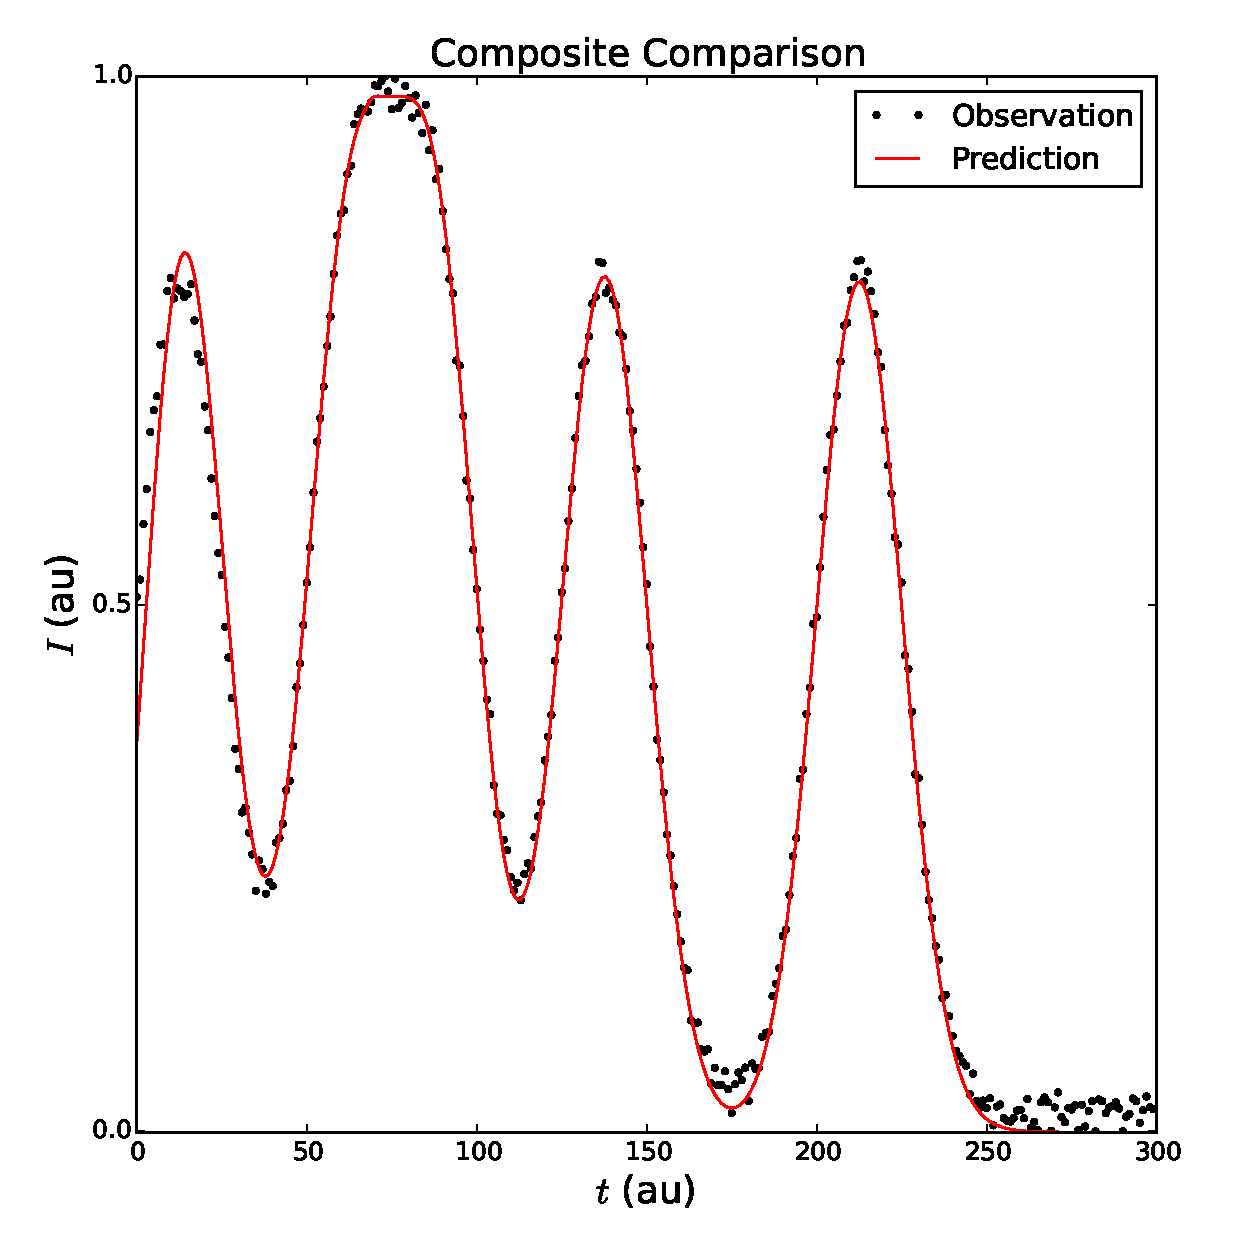
\includegraphics[width=0.5\columnwidth]{figures/ts_total_example.eps}
				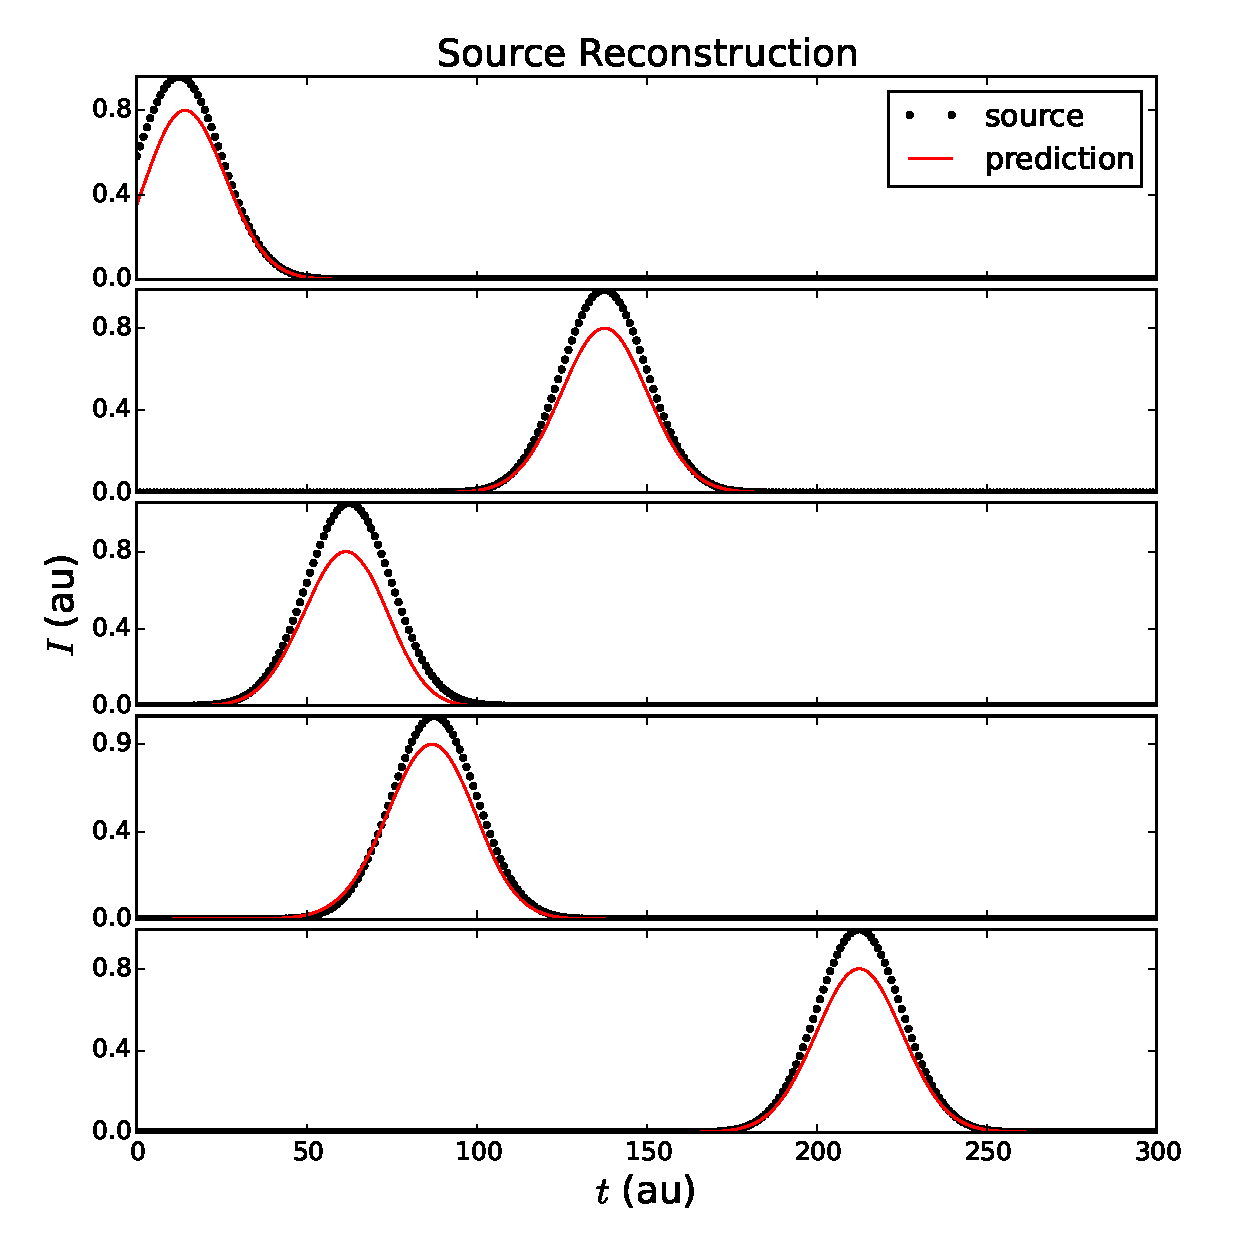
\includegraphics[width=0.5\columnwidth]{figures/ts_source_example.eps}
				\caption{\footnotesize Example factorization for 5 gaussian sources with added noise. Note that NMF is able to recover the two heavily overlapping peaks near $t=75$. Axes are in arbitrary units with amplitude scaled to unity.}
				\label{fig:test_case_1D}
			\end{figure}
		\end{block}
		%%
      \end{column}
	  %Start third column
      \begin{column}{.32\linewidth}
		  %Conclusions block
        \begin{block}{Results}
          \begin{itemize}
          \item NMF algorithm applied to forward-modeled SDO/AIA pixel-averaged time series (Fig. \ref{fig:ar_viz_ts}) for $k\in[10,50]$ 
		  \item In order to estimate number of true sources, fit $d(k)=\alpha e^{-k/\tau_k}$ to $d(T|A)$ as a function of $k$ such that the e-folding length $\tau_k$ is our estimate of the number of sources.
          \end{itemize}
		\begin{figure}
			\subfigure[]{%
			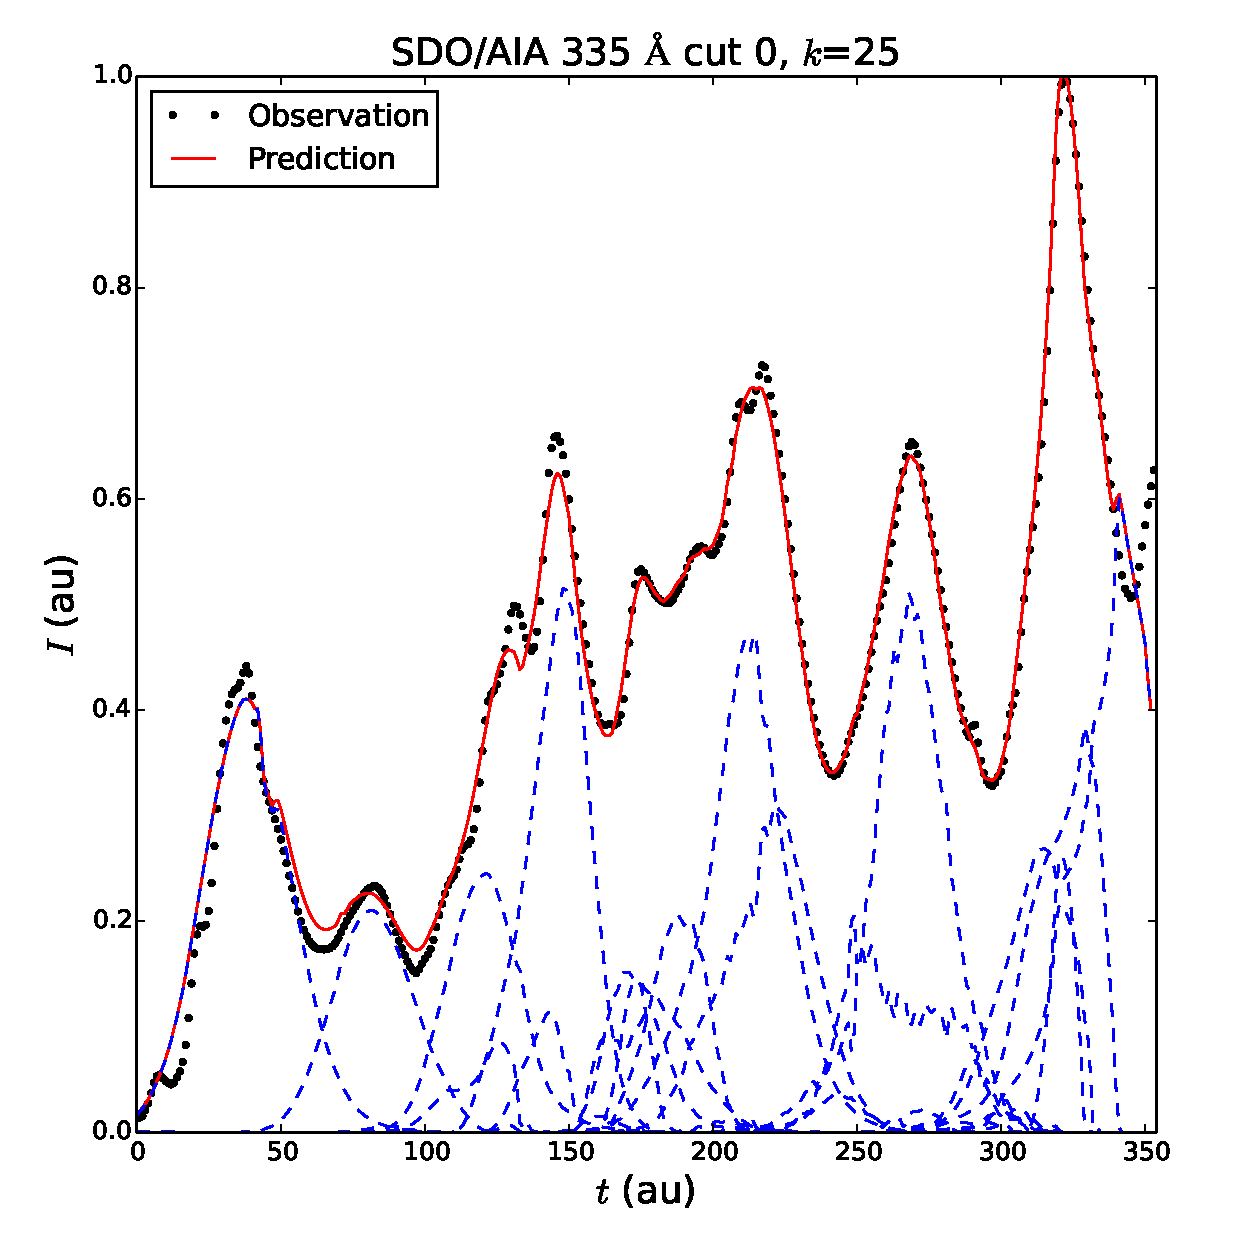
\includegraphics[width=0.49\columnwidth]{figures/channel335_cut0_q25.eps}
			\label{fig:cut0_335_sources}}
			\subfigure[]{%
			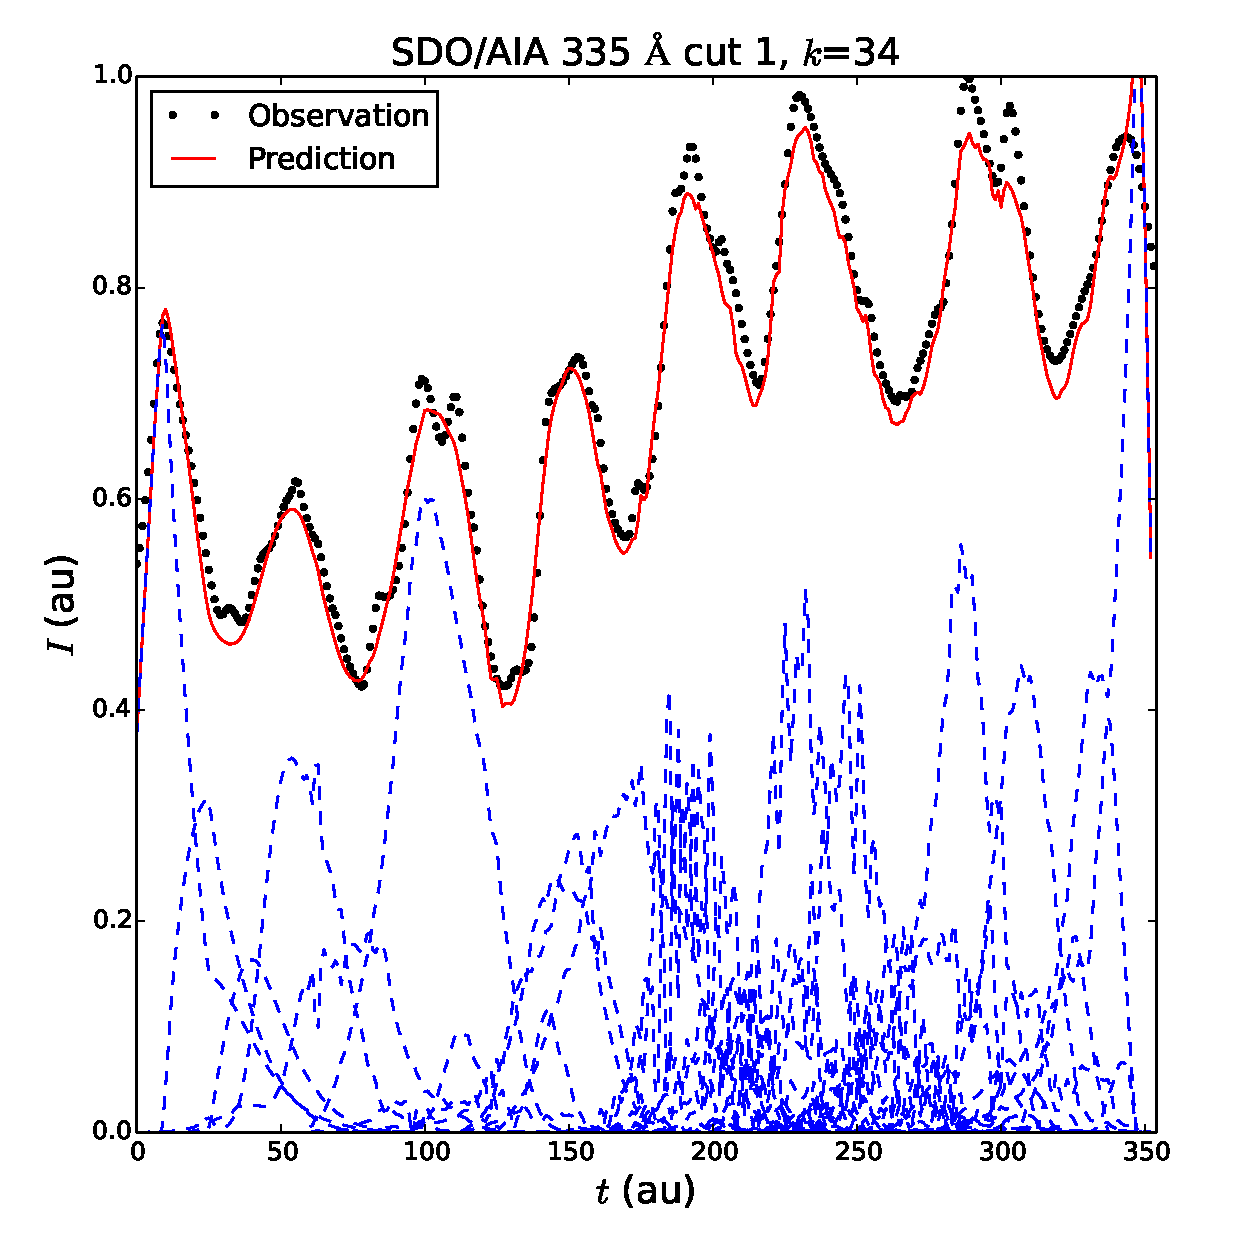
\includegraphics[width=0.49\columnwidth]{figures/channel335_cut1_q34.eps}
			\label{fig:cut1_335_sources}}
			\subfigure[]{%
			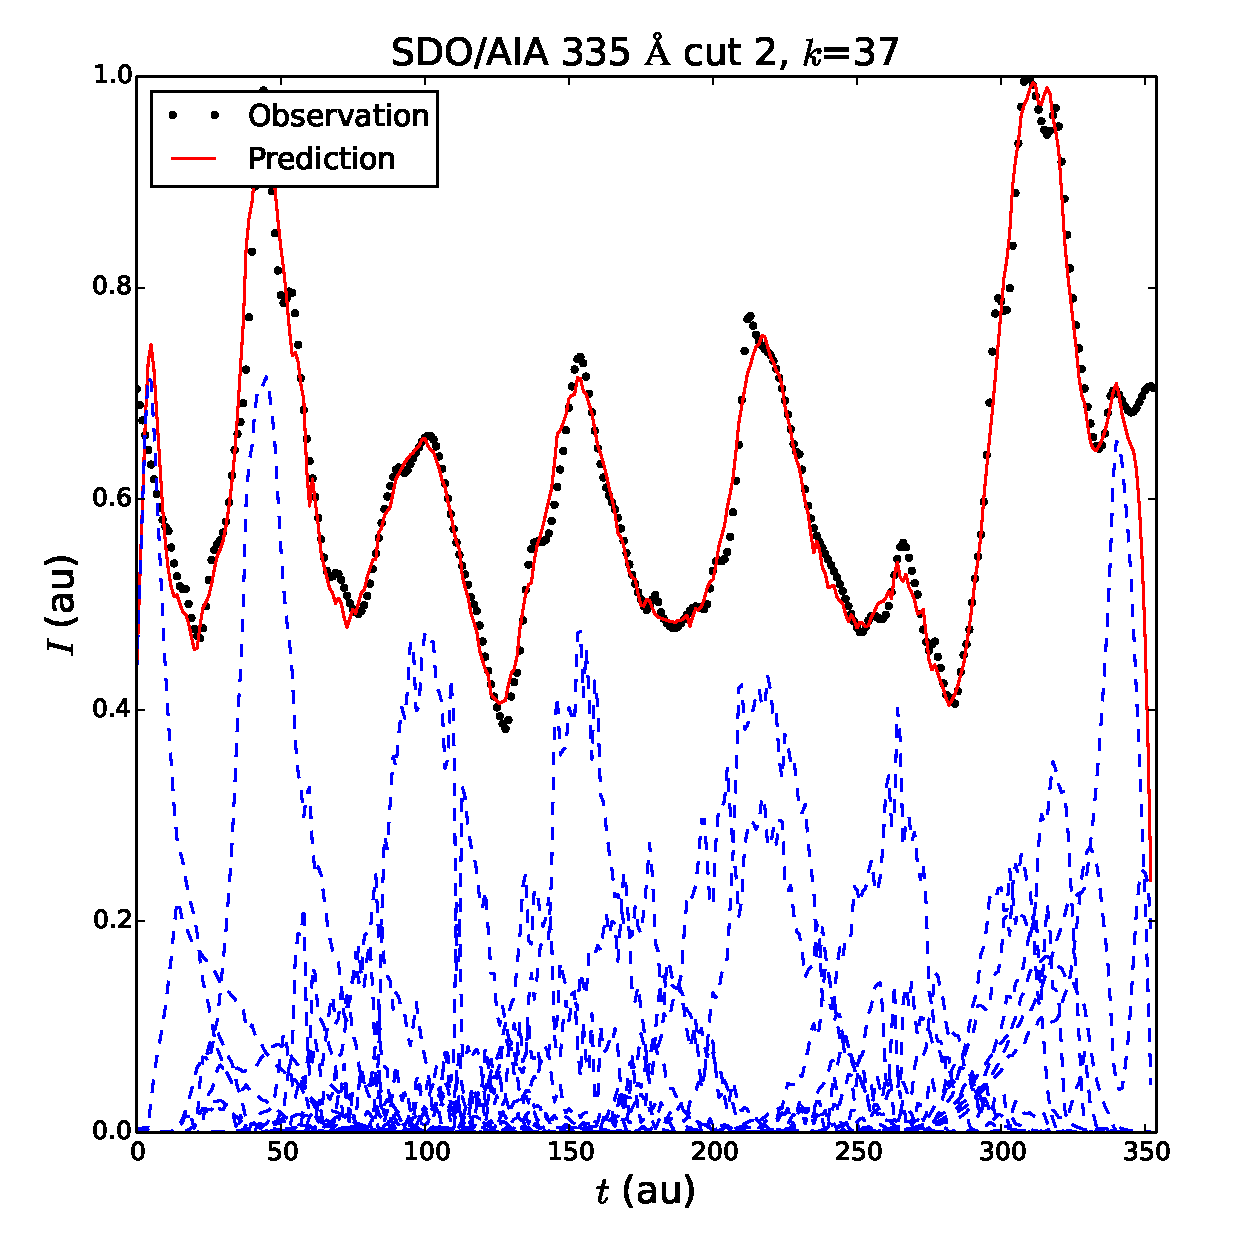
\includegraphics[width=0.49\columnwidth]{figures/channel335_cut2_q37.eps}
			\label{fig:cut2_335_sources}}
			\subfigure[]{%
			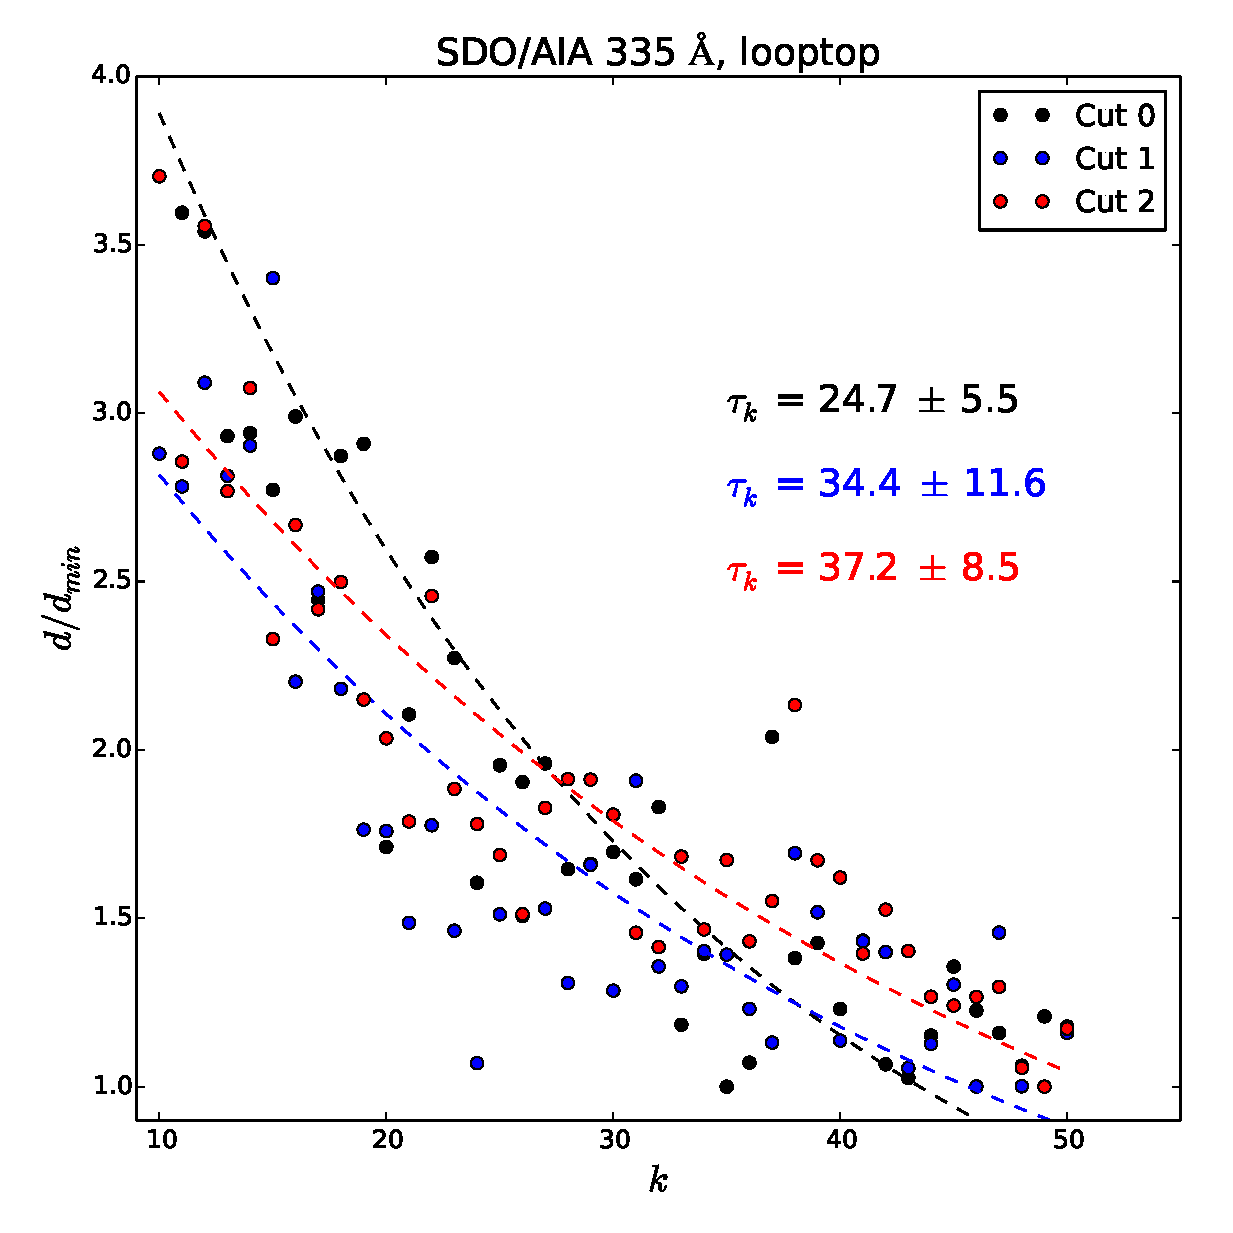
\includegraphics[width=0.49\columnwidth]{figures/nmf_div_comp_335.eps}
			\label{fig:div_comp}}
			\caption{\footnotesize \ref{fig:cut0_335_sources}-\ref{fig:cut2_335_sources} show the total reconstructed light curve plus the estimated underlying sources (in blue) for the light curve sections shown in Fig. \ref{fig:ar_viz_ts}. \ref{fig:div_comp} shows the final value of $d(T|A)$ (normalized to $\min(d(T|A))$ as a function of $k$; dotted lines show the exponential fit.}
		\end{figure}
        \end{block}
		%Future work block
		\begin{block}{Conclusions \& Future Work}
			\begin{itemize}
				\item Expected number of events per cut $=A_{\text{white box}}/A_{AR}\times N_{\text{total}}(=3448)/3\approx86>N_{\text{predicted}}$ for all sections of the 335 \AA~light curve.
				\item As $k$ increases, $d(T|A)$ tends to decrease regardless of number of true sources; testing with gaussian sources(i.e. Fig. \ref{fig:test_case_1D}) will help to address this effect
				\item Single-pixel and filtered forward-modeled emission \citep[see][]{warren_systematic_2012} will provide more conclusive tests.
				\item \alert{True advantage of NMF will be seen in application to 2D AR images} (i.e. Fig.~\ref{fig:ar_viz}); interesting and exciting alternative to traditional detection methods.
			\end{itemize}
			
		\end{block}
	  \begin{block}{References}
	  	\scriptsize
		\bibliographystyle{apj}
	  	\bibliography{references.bib}
	  \end{block}
    \end{column}
	%\begin{columns}[b]
  	%  \begin{column}{0.96\linewidth}
    %
  	%  \end{column}
	\end{columns}
\end{frame}
\end{document}


